

\begin{figure}[!h]
\centering
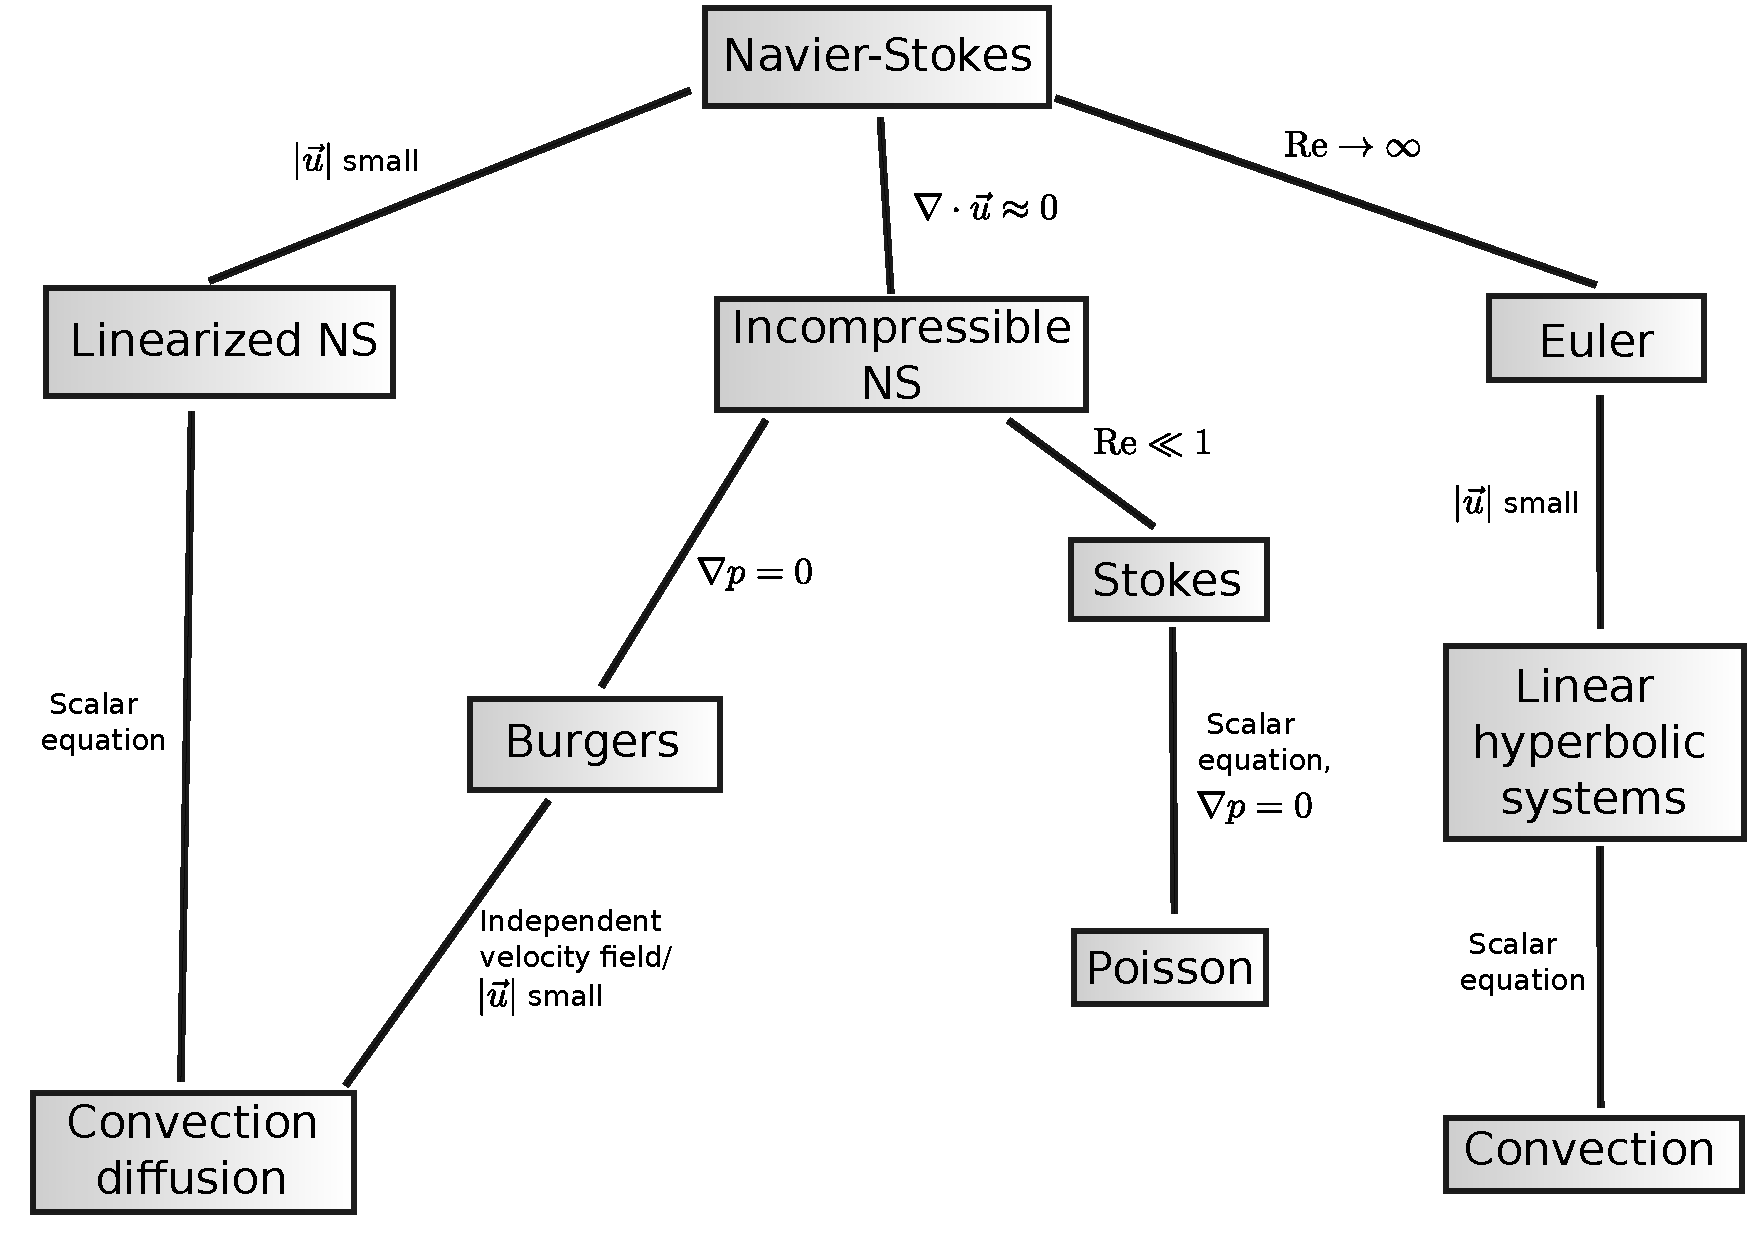
\includegraphics[scale=.45]{figs/CFD_tree.pdf}
\caption{A diagram of common CFD problems and their simplifying assumptions.}
\end{figure}

\section{The compressible Navier-Stokes equations}
\seclab{sec:compNS}

We consider the transient compressible Navier-Stokes equations. For simplicity, we present them in two spatial dimensions. Each equation of the Navier-Stokes system represents the conservation of some physical quantity in the behavior of a fluid inside a general control volume.\footnote{The derivation of the compressible Navier-Stokes equations is a standard result of the Reynolds transport theorem, and can be found in many elementary fluid dynamics books.}

\begin{itemize}
\item{\textbf{Mass conservation}}
\begin{align*}
\pd{\rho}{t} + \div \vecttwo{\rho u }{\rho v} &= 0
\end{align*}

\item{\textbf{Momentum conservation}}
\begin{align*}
\pd{\rho u_1}{t} + \div \left(\vecttwo{\rho u^2+p }{\rho u v} - \boldsymbol \sigma_{1}\right) &=0\\
\pd{\rho u_2}{t} + \div \left(\vecttwo{\rho u v}{\rho v^2+p } - \boldsymbol \sigma_{2}\right) &=0
\end{align*}

\item{\textbf{Energy conservation}}
\begin{align*}
\pd{\rho e}{t} + \div \left(\vecttwo{((\rho e)+p)u}{((\rho e)+p)v} - \boldsymbol \sigma_1 \cdot \boldsymbol u- \boldsymbol \sigma_2 \cdot \boldsymbol u + \vec{q}\right) &=0
\end{align*}
\end{itemize}

We assume our fluid satisfies standard stress laws for $\boldsymbol \sigma$ and $\boldsymbol q$ as well. For viscous stresses $\boldsymbol \sigma$, we assume a Newtonian fluid
\begin{align*}
\sigma_{ij} &= \mu(u_{i,j}+u_{j,i}) + \lambda u_{k,k}\delta_{ij}.
\end{align*}
The coefficients $\lambda$ and $\mu$ are known as the viscosity and bulk viscosity, respectively. The bulk viscosity is often set implicitly through $2\mu + 3\lambda = 0$, known as Stokes' hypothesis. However, since the effect of bulk viscosity can become important for compressible flows, we treat both coefficients separately. In general, $\mu$ and $\lambda$ are functions of temperature, obeying the power law
\[
\mu = \left(\frac{T}{T_0}\right)^\beta,
\]
where $T_0$ is a reference temperature. We choose $\beta = 2/3$ in this case. 

We assume our fluid satisfies Fourier's law, which relates the heat flux $\boldsymbol q$ to the gradient of the temperature through
\begin{align*}
{\boldsymbol q} &= \kappa \grad T,
\end{align*}
where $\kappa$ is generally a function of temperature. 

Finally, we assume our fluid is a thermally and calorically perfect ideal gas. Let $c_p$ and $c_v$ be the specific heats at constant pressure and volume, respectively. Then,
\begin{align*}
p &= (\gamma-1)\rho\iota\\
\iota &= e-\frac{1}{2}(u_1^2+u_2^2)\\
\iota &= c_vT
\end{align*}
where $e$ and $\iota$ are energy and internal energy per unit mass, respectively. 

\todo{write blurb on how comp NS is used - small Re limit}
\todo{write blurb on turbulence}

\subsection{Incompressibility}

\todo{reference Stokes, cite Nate}
\cite{stokesDPG}

\subsection{The linearized Navier-Stokes equations}

The linearized Navier-Stokes equations are the result of small perturbation assumptions applied to the full Navier-Stokes equations. Under such assumptions, the flow is largely uniform, with slight variations that are small compared to the uniform stream velocity. We are interested in the linearized Navier-Stokes equations mainly for mathematical purposes; 

\section{The scalar convection-diffusion equation}

The scalar convection-diffusion problem is the prototypical model problem for solving the full Navier-Stokes equations; most stabilized methods consider first the scalar convection-diffusion equation as a test case before attempting a solution of the full Navier-Stokes equations. As discussed previously, an important feature of the convection-diffusion equation is that solutions can develop  boundary layers, a physical feature found in most applications of interest for compressible flow. 

\todo{add perspective on convection-diffusion}

\subsection{Burgers' equation}

The Burgers' equation is physically derived from the incompressible Navier-Stokes equations under the assumption that $\grad p \approx 0$, or that the pressure field is near constant. A feature of the Burgers' equation not present in convection-diffusion is that, due to the presence of the nonlinear term, it can develop shock discontinuities in its solutions in finite time. 

The Burgers' equation has also been used to study the phenomenon of turbulence; however, the Burgers equation does not exhibit the chaotic nature and sensitivity to initial conditions that characterizes turbulence as observed in the full and incompressible Navier-Stokes equations. In the scope of this dissertation, Burgers shall be used as to test the extension of our numerical method to nonlinear problems. 

\section{The inviscid case}

The Euler equations are a result of neglecting the viscous terms in the Navier-Stokes equations. Physically speaking, these assumptions correspond to the inviscid limit, as well as a particular class of boundary conditions (for example, the wall boundary condition $\boldsymbol u = 0$ does not hold in the inviscid limit). 

\todo{express coupling - Drela's IBL work} \cite{BoeingDrela}
\todo{Express that mathematically, the Euler equations are difficult}

